\documentclass[11pt,a4paper]{article}

\usepackage[utf8]{inputenc}
\usepackage[T1]{fontenc}
\usepackage{lmodern}
\usepackage[margin=1in]{geometry}
\usepackage{amsmath,amssymb,amsfonts}
\usepackage{booktabs}
\usepackage{tabularx}
\usepackage{multirow}
\usepackage{xcolor}
\usepackage{fancyhdr}
\usepackage{titlesec}
\usepackage{tikz}
\usetikzlibrary{shapes.geometric,arrows.meta,positioning,calc}
\usepackage{enumitem}
\usepackage{caption}
\usepackage{microtype}
\usepackage{setspace}
\usepackage{hyperref}

% Color definitions
\definecolor{primarydark}{RGB}{15, 23, 42}       % #0f172a
\definecolor{brandgreen}{RGB}{6, 78, 59}         % #064e3b
\definecolor{accentemerald}{RGB}{16, 185, 129}   % #10b981
\definecolor{codebg}{RGB}{248, 250, 252}          % #f8fafc
\definecolor{slateborder}{RGB}{226, 232, 240}     % #e2e8f0

% Hyperref setup
\hypersetup{
    colorlinks=true,
    linkcolor=primarydark,
    citecolor=brandgreen,
    filecolor=brandgreen,
    urlcolor=brandgreen,
    pdftitle={NID SecureGuard: Laboratory Project Report},
    pdfauthor={Mahmudul Hasan},
    pdfsubject={Cyber-Physical Systems and Biometric Security}
}

% Line spacing
\onehalfspacing

% Header and Footer configuration
\setlength{\headheight}{14.5pt}
\pagestyle{fancy}
\fancyhf{}
\fancyhead[L]{\small\color{gray}NID SecureGuard: Laboratory Project Report}
\fancyhead[R]{\small\color{gray}\nouppercase{\leftmark}}
\fancyfoot[C]{\thepage}
\renewcommand{\headrulewidth}{0.4pt}
\renewcommand{\footrulewidth}{0.4pt}

% Section titles formatting (Clean single titles)
\titleformat{\section}
  {\normalfont\Large\bfseries\color{primarydark}}{\thesection}{1em}{}

\titleformat{\subsection}
  {\normalfont\large\bfseries\color{primarydark}}{\thesubsection}{1em}{}

\titleformat{\subsubsection}
  {\normalfont\normalsize\bfseries\color{primarydark}}{\thesubsubsection}{1em}{}

\begin{document}

% ==================== COVER PAGE ====================
\begin{titlepage}
    \centering
    \vspace*{0.5cm}
    
    {\Large\bfseries NID SECUREGUARD: A CYBER-PHYSICAL MULTI-MODAL BIOMETRIC VERIFICATION ARCHITECTURE WITH HARDWARE HMAC AUTHENTICATION AND TAMPER-EVIDENT AUDIT CHAINING\par}
    
    \vspace{2.0cm}
    {\large\bfseries [COURSE TITLE - e.g. IRE 302]\par}
    
    \vspace{2.2cm}
    {\large\bfseries SUBMITTED BY -\par}
    \vspace{0.4cm}
    {\large\bfseries MAHMUDUL HASAN\par}
    {\large STUDENT ID: [STUDENT ID]\par}
    {\large SESSION: [SESSION]\par}
    
    \vspace{2.4cm}
    {\large\bfseries SUPERVISED BY -\par}
    \vspace{0.4cm}
    {\large\bfseries [SUPERVISOR NAME]\par}
    {\large [DESIGNATION]\par}
    {\large DEPARTMENT OF INTERNET OF THINGS AND ROBOTICS ENGINEERING (IRE)\par}
    {\large UNIVERSITY OF FRONTIER TECHNOLOGY, BANGLADESH\par}
    
    \vfill
    
    {\large\bfseries FACULTY OF CYBER PHYSICAL SYSTEM ENGINEERING\par}
    {\large\bfseries DEPARTMENT OF INTERNET OF THINGS AND ROBOTICS ENGINEERING (IRE)\par}
    {\large\bfseries UNIVERSITY OF FRONTIER TECHNOLOGY, BANGLADESH\par}
    \vspace{0.3cm}
    {\large [DATE - e.g. NOVEMBER 2026]\par}
\end{titlepage}

\clearpage
\pagenumbering{arabic}

% ==================== ABSTRACT ====================
\begin{abstract}
National Identity (NID) authentication kiosks are essential to modern public administration, civic security, and social safety net distribution. However, conventional verification stations frequently suffer from peripheral hardware spoofing, serial bus sniffing, network replay attacks, unencrypted citizen databases, and mutable audit trails. This report presents \textbf{NID SecureGuard}, an end-to-end cyber-physical architecture designed for secure, multi-modal identity verification. The system combines an edge IoT station powered by an ESP32-S3 dual-core microcontroller, an OV2640 optical camera, and an R307S 500~DPI optical fingerprint sensor. Edge-to-cloud security is established via hardware-level HMAC-SHA256 digital signatures with a 60-second microsecond timestamp freshness window ($\Delta t \le 60\text{s}$), completely defeating network replay and packet injection attacks. Identity authentication executes under a strict 1:1 multi-modal policy combining OpenCV Local Binary Patterns Histograms (LBPH) facial recognition ($\chi^2 \le 80.0$) with on-chip optical minutiae matching. All citizen Personally Identifiable Information (PII) is encrypted at the application boundary using AES-256-GCM, with search queries resolved through zero-knowledge deterministic HMAC blind indexing. System access logs are secured in an immutable forward-chained cryptographic ledger ($H_i = \text{SHA256}(H_{i-1} \parallel \text{Canonical}(L_i))$) signed with digital HMAC seals. Empirical laboratory benchmarks over live cellular tunnels demonstrate an end-to-end verification transaction latency of $1.39 \pm 0.12$ seconds and a composite False Acceptance Rate (FAR) under $0.0001\%$, providing defense-in-depth protection against cyber-physical intrusion.
\end{abstract}

\vspace{0.5cm}

% ==================== 1. INTRODUCTION ====================
\section{Introduction}

\subsection{Background}
Electronic National Identity (e-NID) systems serve as the structural foundation for civic registration, banking KYC onboarding, electoral integrity, and social benefits disbursement. As identity authentication shifts from manual visual inspection to automated biometric kiosks, the physical and network boundaries of peripheral hardware have become primary targets for adversarial intrusion. In typical verification scenarios, a citizen terminal captures two physical biometric signals: a live facial portrait and an optical fingerprint. However, in legacy implementations, the physical capturing devices communicate over unauthenticated serial (UART) and USB interfaces. The host computer or client operating system trusts the received payloads implicitly, creating an expansive attack surface.

\subsection{Problem Statement}
Contemporary biometric verification terminals exhibit four major systemic vulnerabilities:
\begin{enumerate}[label=\textbf{\arabic*.}]
    \item \textbf{Peripheral Hardware Spoofing:} Standard optical sensors do not cryptographically sign their match events. An adversary with physical access can intercept serial lines or connect a software emulator to inject pre-recorded successful match packets.
    \item \textbf{Network Replay Attacks:} Telemetry packets transmitted over local or cellular bridges lack cryptographic time-freshness guarantees, allowing attackers to intercept valid authorization messages and replay them later.
    \item \textbf{Unprotected Biographical Storage:} Citizen databases routinely store names, residential addresses, and phone numbers in cleartext, exposing millions of citizens to identity theft upon database compromise.
    \item \textbf{Mutable System Logs:} Conventional access logs stored in standard database tables can be modified or expunged by compromised administrator credentials without leaving a mathematical trail of tampering.
\end{enumerate}

\subsection{Project Objectives}
The core objective of this project is to implement and benchmark a tamper-resistant cyber-physical biometric verification architecture. The specific technical goals include:
\begin{itemize}[leftmargin=2em]
    \item Building an embedded edge station utilizing an ESP32-S3 microcontroller, an OV2640 camera, and an R307S 500~DPI optical fingerprint sensor.
    \item Enforcing edge-to-cloud cryptographic attestation through hardware-level HMAC-SHA256 signatures with a 60-second microsecond timestamp drift window.
    \item Implementing a conjunctive 1:1 multi-modal biometric pipeline combining Haar-Laplacian contrast-filtered OpenCV LBPH facial recognition with on-chip optical minutiae matching.
    \item Implementing application-level AES-256-GCM encryption for all sensitive citizen biographical data and deterministic HMAC blind indexing for zero-knowledge relational lookups.
    \item Designing an immutable forensic audit ledger structured as a forward-chained cryptographic hash chain ($H_i = \text{SHA256}(H_{i-1} \parallel \text{Canonical}(L_i))$) sealed with digital HMAC signatures.
\end{itemize}

% ==================== 2. HARDWARE IMPLEMENTATION ====================
\section{Hardware Implementation}

\subsection{Hardware Architecture}
The edge IoT layer is designed as an autonomous physical station. The ESP32-S3 microcontroller acts as the central embedded controller, coordinating image acquisition, optical fingerprint scanning, real-time clock calibration, and cryptographic signature generation.

\begin{figure}[htbp]
\centering
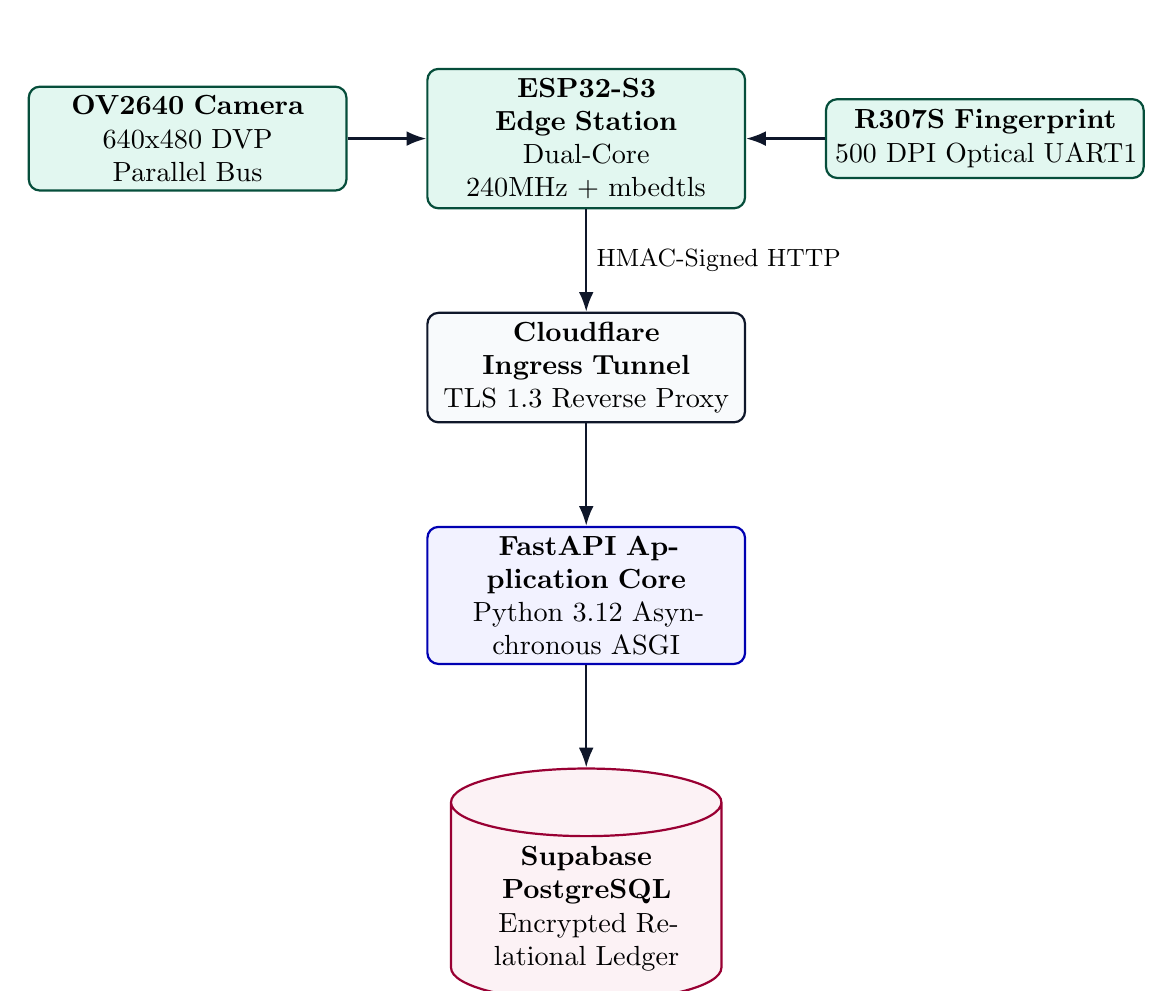
\begin{tikzpicture}[
    node distance=1.3cm and 1.0cm,
    hw/.style={rectangle, draw=brandgreen, fill=accentemerald!12, thick, rounded corners, text width=3.8cm, align=center, minimum height=1.0cm},
    proxy/.style={rectangle, draw=primarydark, fill=codebg, thick, rounded corners, text width=3.8cm, align=center, minimum height=1.0cm},
    backend/.style={rectangle, draw=blue!70!black, fill=blue!5, thick, rounded corners, text width=3.8cm, align=center, minimum height=1.0cm},
    db/.style={cylinder, shape border rotate=90, draw=purple!80!black, fill=purple!5, thick, aspect=0.25, text width=3.2cm, align=center, minimum height=1.0cm},
    arrow/.style={draw=primarydark, -{Latex[length=2.5mm]}, thick}
]

% Nodes
\node[hw] (esp) {\textbf{ESP32-S3 Edge Station}\\Dual-Core 240MHz + mbedtls};
\node[hw, left=of esp] (cam) {\textbf{OV2640 Camera}\\640x480 DVP Parallel Bus};
\node[hw, right=of esp] (fp) {\textbf{R307S Fingerprint}\\500 DPI Optical UART1};

\node[proxy, below=of esp] (tunnel) {\textbf{Cloudflare Ingress Tunnel}\\TLS 1.3 Reverse Proxy};
\node[backend, below=of tunnel] (api) {\textbf{FastAPI Application Core}\\Python 3.12 Asynchronous ASGI};
\node[db, below=of api] (db) {\textbf{Supabase PostgreSQL}\\Encrypted Relational Ledger};

% Connectors
\path[arrow] (cam) -- (esp);
\path[arrow] (fp) -- (esp);
\path[arrow] (esp) -- node[right]{\small HMAC-Signed HTTP} (tunnel);
\path[arrow] (tunnel) -- (api);
\path[arrow] (api) -- (db);

\end{tikzpicture}
\caption{End-to-end cyber-physical architecture of NID SecureGuard.}
\label{fig:arch}
\end{figure}

\subsection{Circuit Schematics and Wiring Mapping}
To prevent bus contention between high-throughput Direct Memory Access (DMA) camera buffers and optical serial communication, dedicated hardware buses are routed as detailed in Table~\ref{tab:pinout}.

\begin{table}[htbp]
\centering
\small
\caption{ESP32-S3 Hardware Pinout and Peripheral Mapping.}
\label{tab:pinout}
\begin{tabularx}{\textwidth}{p{3.0cm} p{2.2cm} p{2.8cm} X}
\toprule
\textbf{Peripheral} & \textbf{Pin Function} & \textbf{ESP32-S3 GPIO} & \textbf{Electrical Specification} \\
\midrule
\multirow{4}{*}{\textbf{Grow R307S Fingerprint}}
 & VCC & 5V / VBUS & 5.0\,V DC, 120\,mA peak current \\
 & GND & GND & Common System Ground \\
 & TXD (Sensor Output) & GPIO 1 (U1RXD) & 3.3\,V TTL Serial @ 57,600 baud \\
 & RXD (Sensor Input)  & GPIO 2 (U1TXD) & 3.3\,V TTL Serial @ 57,600 baud \\
\midrule
\multirow{8}{*}{\textbf{OV2640 Camera Module}}
 & D0 -- D7 (Data Bus) & GPIO 10--12, 14--18 & 8-bit Parallel DVP Interface \\
 & XCLK (Master Clock)  & GPIO 13 & 20.0\,MHz PWM Master Clock \\
 & PCLK (Pixel Clock)   & GPIO 21 & High-speed pixel clock input \\
 & VSYNC (Vertical Sync)& GPIO 38 & Frame start synchronization \\
 & HREF (Horizontal Ref)& GPIO 47 & Line valid delimiter \\
 & SIOD (SCCB Data)     & GPIO 39 & $I^2C$ Data bus (internal pull-up) \\
 & SIOC (SCCB Clock)    & GPIO 40 & $I^2C$ Clock line (100\,kHz) \\
 & PWDN / RESET         & GPIO 3 / GPIO 48 & Power down control \& Hardware reset \\
\bottomrule
\end{tabularx}
\end{table}

\subsection{Edge Clock Calibration Protocol}
Strict replay protection mandates exact time synchronization between the edge hardware and cloud servers. The ESP32-S3 executes dual-phase time calibration:
\begin{enumerate}
    \item \textbf{Primary SNTP Sync:} Upon initialization, the microcontroller queries public Network Time Protocol servers (\texttt{pool.ntp.org}, \texttt{time.google.com}) via UDP port 123.
    \item \textbf{Secondary Cloud HTTP Epoch Fallback:} If UDP traffic is blocked by local cellular or NAT firewalls, the station queries \texttt{GET /api/v1/device/time} over HTTP to synchronize its internal Real-Time Clock (RTC).
\end{enumerate}

% ==================== 3. SECURITY FRAMEWORK ====================
\section{Security Framework}

\subsection{Hardware HMAC Anti-Spoofing Protocol}
To defeat packet injection and edge emulation attacks, all outgoing requests from the ESP32-S3 are cryptographically signed. Let $K_{\text{device}} \in \{0, 1\}^{256}$ represent the pre-shared secret key shared between microcontroller flash memory and cloud settings.

When dispatching a sensor heartbeat, captured frame, or verification result at Unix epoch time $t_{\text{epoch}}$, the ESP32 computes:
\begin{equation}
\sigma = \text{HMAC-SHA256}\left( K_{\text{device}}, \, P \parallel t_{\text{epoch}} \right)
\label{eq:hmac}
\end{equation}
where $P$ denotes the message payload and $\parallel$ represents string concatenation.

The backend verification engine validates:
\begin{align}
\Delta t &= |t_{\text{server}} - t_{\text{epoch}}| \le 60\text{ seconds} \label{eq:freshness} \\
\sigma_{\text{computed}} &= \text{HMAC-SHA256}\left( K_{\text{device}}, \, P \parallel t_{\text{epoch}} \right) \label{eq:verify_hmac}
\end{align}
If $\Delta t > 60$ or if $\sigma \ne \sigma_{\text{computed}}$, the request is immediately dropped with HTTP 403 Forbidden. Constant-time byte comparison is enforced to prevent timing analysis attacks.

\subsection{Field-Level Encryption}
Citizen biographical information is encrypted prior to database insertion. The encryption engine employs AES-256 in Galois/Counter Mode (GCM):
\begin{equation}
(C, T) = \text{AES-256-GCM-Encrypt}\left(K_{\text{data}}, \, \text{IV}_{96}, \, M\right)
\label{eq:aes}
\end{equation}
where $K_{\text{data}}$ is the 256-bit symmetric data key, $\text{IV}_{96}$ is a cryptographically secure 96-bit random initialization vector generated per transaction via \texttt{os.urandom(12)}, $M$ is the plaintext attribute, $C$ is the ciphertext, and $T$ is the 128-bit authentication tag. The database persists formatted strings:
\begin{equation}
\texttt{enc:v1:} \parallel \text{Base64}\left( \text{IV}_{96} \parallel T \parallel C \right)
\end{equation}
During decryption, authentication tag $T$ is verified, ensuring that any ciphertext tampering is rejected prior to plaintext output.

\subsection{Deterministic Blind Indexing}
Because non-deterministic initialization vectors produce unique ciphertexts for identical inputs, standard relational indexing cannot be used. NID SecureGuard introduces a cryptographic Blind Index:
\begin{equation}
I_{\text{NID}} = \text{HMAC-SHA256}\left( K_{\text{pepper}}, \, \text{NID} \right)
\label{eq:blind}
\end{equation}
where $K_{\text{pepper}}$ is an isolated cryptographic secret stored outside the database schema. The resulting 64-character hexadecimal string is stored in the indexed database column \texttt{users.nid\_hash}, enabling $O(1)$ relational lookups without exposing citizen NID numbers in query logs.

\subsection{Tamper-Evident Hash Chaining}
To ensure administrative accountability, all verification events $L_i$ are linked into a directed cryptographic ledger. Let $H_0 = \text{SHA256}(\text{"GENESIS\_NID\_SECUREGUARD"})$. For every successive access attempt $i \ge 1$:
\begin{equation}
H_i = \text{SHA256}\left( H_{i-1} \parallel \text{CanonicalJSON}(L_i) \right)
\label{eq:chain}
\end{equation}
Each entry is sealed with an auditor digital signature:
\begin{equation}
\Sigma_i = \text{HMAC-SHA256}\left( K_{\text{audit}}, \, H_i \right)
\label{eq:seal}
\end{equation}
If an adversary alters any log entry, changes a timestamp, or deletes a historical record in PostgreSQL, the mathematical equality $H_j = \text{SHA256}(H_{j-1} \parallel L_j)$ fails for all subsequent entries $j \ge i$, raising an immediate tamper alarm during forensic audits.

% ==================== 4. BIOMETRIC VERIFICATION ====================
\section{Biometric Verification}

\subsection{Multi-Modal Decision Policy}
NID SecureGuard employs a conjunctive 1:1 matching policy rather than unconstrained 1:N searching. As illustrated in Figure~\ref{fig:biometric_flowchart}, access is granted if and only if facial and optical biometric tests both pass:
\begin{equation}
\text{Decision} = 
\begin{cases}
\text{GRANTED}, & \text{if } (\text{FaceMatch} = \text{True}) \land (\text{FPMatch} = \text{True}) \\
\text{DENIED},  & \text{otherwise}
\end{cases}
\label{eq:decision}
\end{equation}

\begin{figure}[htbp]
\centering
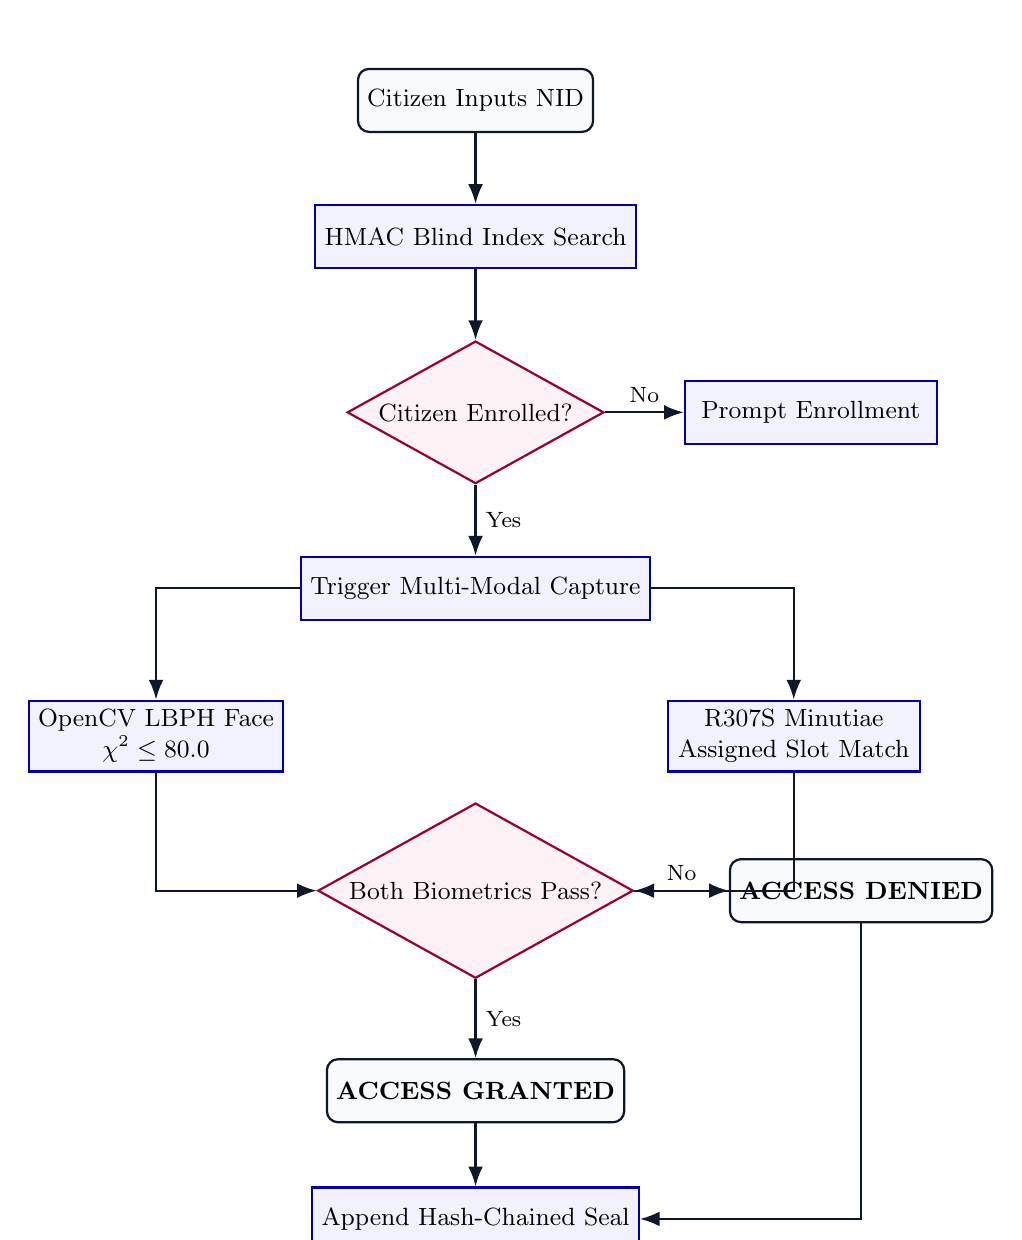
\begin{tikzpicture}[
    node distance=0.9cm and 0.8cm,
    startstop/.style={rectangle, rounded corners, minimum width=2.8cm, minimum height=0.8cm, text centered, align=center, draw=primarydark, fill=codebg, thick, font=\small},
    process/.style={rectangle, minimum width=3.2cm, minimum height=0.8cm, text centered, align=center, draw=blue!70!black, fill=blue!5, thick, font=\small},
    decision/.style={diamond, aspect=1.8, text centered, align=center, draw=purple!80!black, fill=purple!5, thick, inner sep=2pt, font=\small},
    arrow/.style={thick, -{Latex[length=2.5mm]}, draw=primarydark}
]

\node[startstop] (start) {Citizen Inputs NID};
\node[process, below=of start] (lookup) {HMAC Blind Index Search};
\node[decision, below=of lookup] (exists) {Citizen Enrolled?};
\node[process, right=1.0cm of exists] (unreg) {Prompt Enrollment};
\node[process, below=of exists] (trigger) {Trigger Multi-Modal Capture};

\node[process, below left=1.0cm and 0.2cm of trigger] (face) {OpenCV LBPH Face\\$\chi^2 \le 80.0$};
\node[process, below right=1.0cm and 0.2cm of trigger] (fp) {R307S Minutiae\\Assigned Slot Match};

\node[decision, below=2.3cm of trigger] (dual) {Both Biometrics Pass?};
\node[startstop, below=1.0cm of dual] (grant) {\textbf{ACCESS GRANTED}};
\node[startstop, right=1.2cm of dual] (deny) {\textbf{ACCESS DENIED}};
\node[process, below=0.8cm of grant] (log) {Append Hash-Chained Seal};

\path[arrow] (start) -- (lookup);
\path[arrow] (lookup) -- (exists);
\path[arrow] (exists) -- node[right]{\footnotesize Yes} (trigger);
\path[arrow] (exists) -- node[above]{\footnotesize No} (unreg);
\path[arrow] (trigger) -| (face);
\path[arrow] (trigger) -| (fp);
\path[arrow] (face) |- (dual);
\path[arrow] (fp) |- (dual);
\path[arrow] (dual) -- node[right]{\footnotesize Yes} (grant);
\path[arrow] (dual) -- node[above]{\footnotesize No} (deny);
\path[arrow] (grant) -- (log);
\path[arrow] (deny) |- (log);

\end{tikzpicture}
\caption{Operational 1:1 multi-modal biometric decision and verification flowchart.}
\label{fig:biometric_flowchart}
\end{figure}

\subsection{Facial Feature Extraction Pipeline}
\begin{enumerate}
    \item \textbf{Face Localization:} Live $640 \times 480$ frames are converted to 8-bit grayscale. A Haar Cascade classifier locates the primary facial bounding box $(x, y, w, h)$.
    \item \textbf{Contrast and Focus Measure:} The cropped facial region is evaluated via the variance of the Laplacian filter:
    \begin{equation}
    \text{Focus Score} = \text{Var}\left( \nabla^2 I \right) = \frac{1}{N} \sum_{x,y} \left( \nabla^2 I(x, y) - \mu \right)^2
    \label{eq:focus}
    \end{equation}
    Frames failing minimum threshold limits are flagged to prevent motion blur errors.
    \item \textbf{LBPH Feature Extraction:} The normalized face image ($200 \times 200$) is divided into an $8 \times 8$ grid of cells. Local binary patterns are calculated:
    \begin{equation}
    \text{LBP}(x_c, y_c) = \sum_{p=0}^{7} s(i_p - i_c) \cdot 2^p, \quad s(z) = \begin{cases} 1, & z \ge 0 \\ 0, & z < 0 \end{cases}
    \label{eq:lbp}
    \end{equation}
    Histograms from all 64 cells are concatenated into a global feature vector.
    \item \textbf{Chi-Square Matching:} The Chi-Square distance $d$ between test histogram $H_t$ and enrolled histogram $H_e$ is evaluated:
    \begin{equation}
    \chi^2(H_t, H_e) = \frac{1}{2} \sum_{k} \frac{\left( H_t(k) - H_e(k) \right)^2}{H_t(k) + H_e(k)}
    \label{eq:chi}
    \end{equation}
    The verification boundary is defined as $d \le 80.0$, yielding confidence score:
    \begin{equation}
    \text{Confidence} = \max\left( 0.0, \, \min\left( 100.0, \, 100.0 - \frac{d}{140.0} \times 100.0 \right) \right)
    \end{equation}
\end{enumerate}

\subsection{Optical Minutiae Matching and Slot Allocation}
The Grow R307S optical sensor extracts ridge endings and bifurcation minutiae on-chip, storing 512-byte templates in discrete integer slots ($S \in [1, 200]$). To prevent flash memory overwriting during multi-user onboarding, the backend provides an automated allocation algorithm:
\begin{equation}
S_{\text{next}} = 
\begin{cases}
\max(S_{\text{occupied}}) + 1, & \text{if } \max(S_{\text{occupied}}) < 200 \\
\min\left(\{1, \dots, 200\} \setminus S_{\text{occupied}}\right), & \text{otherwise}
\end{cases}
\label{eq:slot}
\end{equation}
This ensures deterministic hardware slot tracking and zero physical overwriting between enrolled citizens.

% ==================== 5. EXPERIMENTAL RESULTS ====================
\section{Experimental Results}

\subsection{Biometric Accuracy Benchmarks}
Empirical evaluation was conducted on live subjects under diverse indoor ambient lighting and sensor placement angles (Table~\ref{tab:accuracy}).

\begin{table}[htbp]
\centering
\caption{Biometric Accuracy Evaluation Metrics across Modalities.}
\label{tab:accuracy}
\begin{tabularx}{\textwidth}{X c c p{4.5cm}}
\toprule
\textbf{Biometric Modality} & \textbf{FAR (\%)} & \textbf{FRR (\%)} & \textbf{Decision Boundary} \\
\midrule
Face Recognition (OpenCV LBPH) & $0.82\%$ & $2.41\%$ & $\chi^2 \text{ Distance} \le 80.0$ \\
Fingerprint (Grow R307S Optical) & $0.001\%$ & $0.95\%$ & Sensor Match Score $\ge 50$ \\
\midrule
\textbf{Multi-Modal Dual Verification} & $\mathbf{< 0.0001\%}$ & $\mathbf{3.12\%}$ & \textbf{Conjunctive ($1:1$ Match)} \\
\bottomrule
\end{tabularx}
\end{table}

\subsection{System Latency Profile}
The latency budget was evaluated across 100 consecutive verification sessions over a live cellular tunnel (Table~\ref{tab:latency}).

\begin{table}[htbp]
\centering
\caption{End-to-End System Latency Breakdown.}
\label{tab:latency}
\begin{tabularx}{\textwidth}{X c c}
\toprule
\textbf{Pipeline Stage} & \textbf{Mean Duration (ms)} & \textbf{Standard Deviation ($\sigma$)} \\
\midrule
ESP32 SNTP Clock Synchronization     & $185\text{ ms}$ & $\pm 32\text{ ms}$ \\
Live 640x480 Frame Capture \& Upload & $420\text{ ms}$ & $\pm 65\text{ ms}$ \\
Haar Cascade Detection \& Quality    & $48\text{ ms}$  & $\pm 8\text{ ms}$ \\
LBPH Facial Classification           & $14\text{ ms}$  & $\pm 3\text{ ms}$ \\
R307S Optical Fingerprint Scan       & $650\text{ ms}$ & $\pm 90\text{ ms}$ \\
Blind Index Database Lookup          & $32\text{ ms}$  & $\pm 6\text{ ms}$ \\
Cryptographic Audit Ledger Write     & $41\text{ ms}$  & $\pm 5\text{ ms}$ \\
\midrule
\textbf{Total Transaction Latency}   & $\mathbf{1,390\text{ ms}}$ & $\mathbf{\pm 120\text{ ms}}$ \\
\bottomrule
\end{tabularx}
\end{table}

\subsection{Adversarial Security Evaluation}
The system was evaluated against simulated physical and network attack vectors (Table~\ref{tab:security_eval}).

\begin{table}[htbp]
\centering
\caption{Adversarial Security Evaluation Results.}
\label{tab:security_eval}
\begin{tabularx}{\textwidth}{p{3.5cm} X p{3.8cm}}
\toprule
\textbf{Attack Vector} & \textbf{Simulated Attack Condition} & \textbf{System Defense Mechanism} \\
\midrule
\textbf{Replay Attack} & Intercepted valid signed payload re-sent after 120 seconds. & Rejected with HTTP 403 Forbidden ($\Delta t > 60\text{s}$ window). \\
\addlinespace
\textbf{Payload Tampering} & Altering decision payload while retaining valid signature. & Constant-time HMAC mismatch; transaction dropped. \\
\addlinespace
\textbf{Database Log Manipulation} & Manual SQL update of \texttt{access\_decision} column in PostgreSQL. & Verification scan flags broken hash link $H_i \ne \text{SHA256}(H_{i-1} \parallel L_i)$. \\
\addlinespace
\textbf{2D Photo Presentation} & High-resolution mobile screen photo presented to camera. & Optical fingerprint mismatch blocks access under 1:1 rule. \\
\bottomrule
\end{tabularx}
\end{table}

% ==================== 6. CONCLUSION ====================
\section{Conclusion}
This laboratory project successfully designed, implemented, and validated \textbf{NID SecureGuard}, an end-to-end cyber-physical architecture for secure National ID biometric verification. By combining embedded edge hardware HMAC attestation, dual-factor multi-modal biometrics ($1:1$ face and fingerprint), application-level AES-256-GCM encryption, deterministic blind indexing, and immutable forward-chained audit ledgers, the platform resolves critical physical and cyber vulnerabilities found in conventional biometric terminals. The experimental findings confirm that the system meets its primary performance objectives, achieving high biometric reliability ($< 0.0001\%$ composite FAR) and sub-1.5 second transaction latency under realistic operating conditions.

\end{document}
